\section{Physical dnd biogeochemical response to ENSO variability}
\label{sec:pisces}

The ocean fish biomass is strongly influenced by the physical and geochemical state of the ocean. Therefore, a good understanding of how the ocean responds to ENSO variability is necessary to understand how the signal propagates to the higher trophic levels. The aim of the present section is to describe the response of the NEMO-Pisces model to ENSO variability. \\

\subsection{Covariance analysis}

As a first step, the Ocean Nino Index (ONI\footnote{\url{https://www.cpc.ncep.noaa.gov/data/indices/oni.ascii.txt}}) has been compared with the simulated one, in order to determine whether the timing of simulated ENSO events is consistent with the observed one. The correlation coefficient between the two monthly time-series over the overlapping period (1958-2018) is $0.94$, which gives confidence in the model ability to reproduce the observed ENSO variability. \\

In order to infer the spatial patterns of the physical and biogeochemical response to ENSO variability, covariance between the ONI index and the NEMO-Pisces field anomalies have been computed. 
Since the main focus is on the interannual variability, the covariances are applied on yearly time series. The ONI index has been averaged over boreal winter (from November to January), when most of the ENSO variability occurs. In order to insure continuity over the winter months, when ENSO variability usually peaks, yearly means of physical and biogeochemical variables have been computed from May (year $y$) to April (year $y + 1$), as done in \cite{racaultImpactNinoVariability2017}. Then, the obtained time-series have been detrended.\\

The correlation between the ONI index and the sea-surface temperature is shown in figure \ref{fig:cov-sst}. For comparison, the same analysis has been performed with the Hadley SST dataset \citep{raynerGlobalAnalysesSea2003}
The covariance patterns are very similar between Hadley and simulated SST, with warm anomalies (1\degree C) centerred at the equator and extending from 0 to 90E and from 10S to 10N.\ 
The covariance along the equatorial temperature section (figure \ref{fig:cov-prof}a) shows that the maximum temperature anomalies is at around 50m depth at a longitude of 70E. Negative anomalies (-0.8\degree C) are located on the western part of the basin (20W). This dipolar structure is consistent with a shoaling of the thermocline in the west and a deepening in the east.\\

Oxygen covariance patterns shows an increase in the oxygen concentration in the eastern part of the basin (90E) between 0 and 200m. This increase of oxygen concentration 
is consistent with shoaling of the Oxygen Minimum Zone during \nino\ conditions associated with vertical displacements of the thermocline \citep{leungENSODrivesNearsurface2019, espinoza-morriberonOxygenVariabilityENSO2019}. \\

Covariance patterns for phytoplankton variables show that nano-phytoplankton and diatoms (figures \ref{fig:cov-prof}c and \ref{fig:cov-prof}d) respond in different ways to ENSO variability. Small phytoplankton shows negative anomalies between 0 and 80E in near the surface, and positive anomalies at depth (100m). On the other hand, diatoms show negative anomalies which are confined mainly near the surface in the eastern pacific (80E).\\

Zooplankton shows, as nano-phytoplankton, a decrease at the surface, and an 
increase at lower depth, the latter being more pronounced for micro-zooplankton than for meso-zooplankton (figures \ref{fig:cov-prof}e and \ref{fig:cov-prof}f). The strongest negative anomalies 
are located near the equator for micro-zooplankton, while they are located at around 90E for meso-zooplankton. 
Interestingly, the covariance patterns of nano-phytoplankton and micro-zooplankton on the one hand, and of diatoms and meso-zooplankton on the other hand, bear strong resemblance (compare figures \ref{fig:cov-prof}c-\ref{fig:cov-prof}e and \ref{fig:cov-prof}d-\ref{fig:cov-prof}f). \warn{Possibly something related with the size????}\\

\begin{figure}[h!]
	\centering
	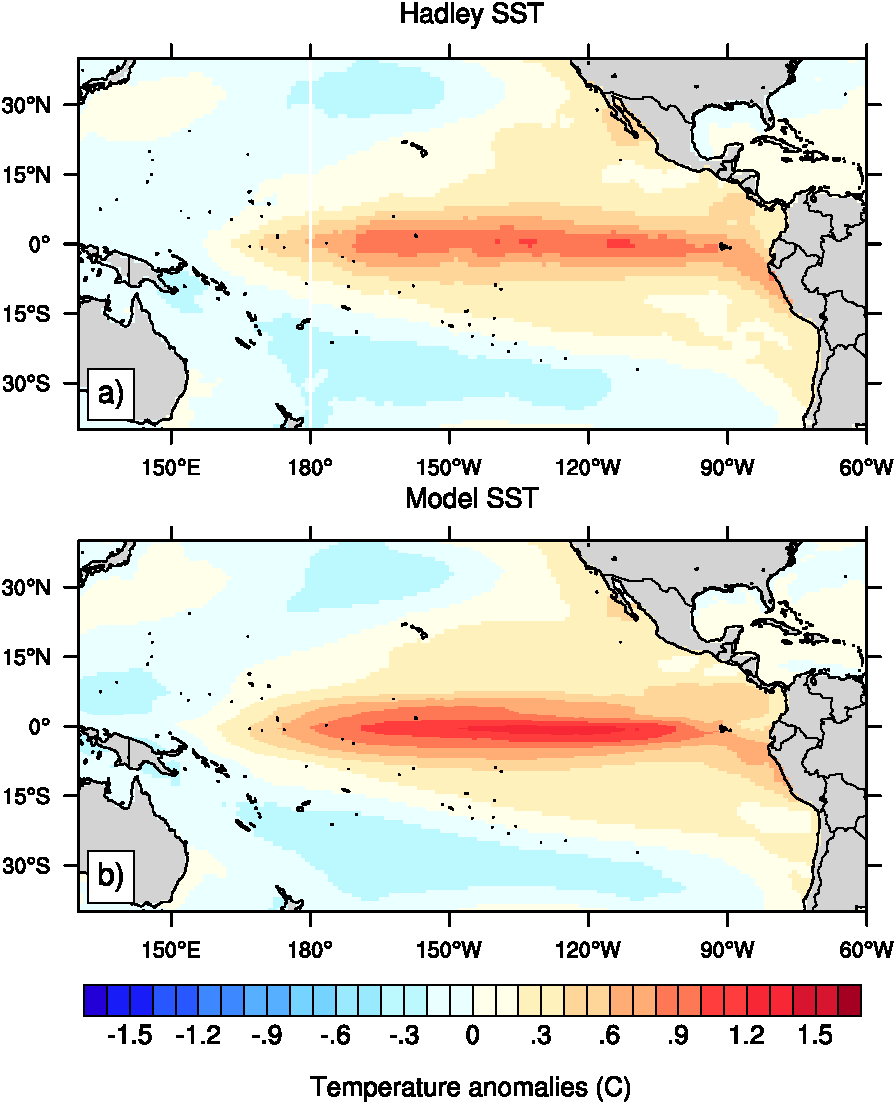
\includegraphics[scale=0.75] {figs/covariance_maps_hadley_model.pdf}
	\caption{Covariance between winter ONI index and Hadley (top) and simulated (bottom) yearly SST anomalies.}
	\label{fig:cov-sst}
\end{figure}

\begin{figure}[h!]
	\centering
	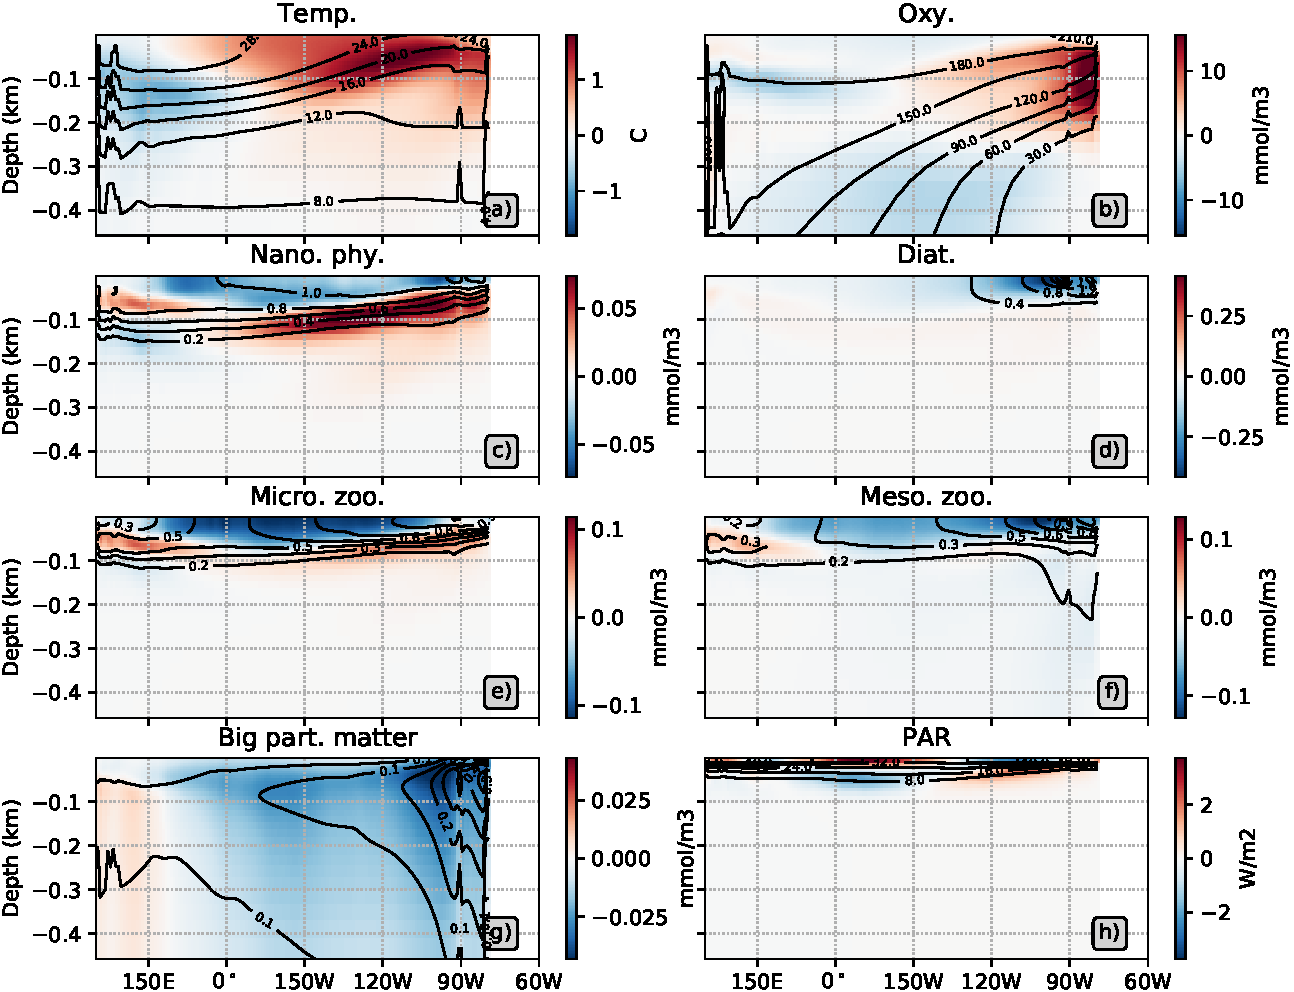
\includegraphics[scale=0.5] {figs/covariance_profiles.pdf}
	\caption{Covariance between winter ONI index and NEMO-Pisces physical and geochemical variables averaged between 2N and 2S. The mean value is show in black contour lines.}
	\label{fig:cov-prof}
\end{figure}

\clearpage

\subsection{Transient response to \nino\ events}

In order to analyse the transient response to \nino\ events, composite analysis has been performed over the most prominent \nino\ years. The latter have been determined as the years durinh which the ONI index averaged from October to December exceeds 1. The obtained years are 1963, 1965, 1972, 1982, 1986, 1987, 1991, 1997, 2002, 2009, and 2015. Because the 1986 \nino\ event extends over two years, 1986 has been removed from the analysis in order to count it only once.\\
 
Monthly anomalies (i.e. seasonal cycle removed) have been averaged from January of the \nino\ years ($Y$) to December of the next two years ($Y + 2$). Composite analysis has first been performed on the physical and biogeochemical averaged over the top 200m of the water column and between 2N and 2S. \\

Warm temperature anomalies (figure \ref{fig:hov-pisces}a) seem to originate at around 15E at the onset of \nino and propagate eastward. The maximum warm anomalies are locateds at around 60E and occurr during the december month of the \nino\ event. Cold anomalies are weaker than warm ones and are at their maximum 10 months after the onset of the \nino\ event, at around 40E.
Contrary to temperature, the oxygen signature of \nino\ events (figure \ref{fig:hov-pisces}b) is limited to the eastern part of the domain, where the \omz\ is situated. At the onset of \nino , oxygen increases sharply (20 $mmol.m^{-3}$). However, around 4 months and 12 months after the \nino\ occurs, the oxygen anomalies are negative and reach -20 $mmol.m^{-3}$. The increase of oxygen can be explained by the shallowing of the highly oxygenated thermocline under \nino\ conditions. \warn{What causes the oxygen decrease? Consumption by plankton? Reduction of PHY, hence no more photo? cf. likeness of O2 and PHY \hov .}.\\

Regarding the response of carbon concentrations, the response of \phy\ and \zoo on the one hand (figures \ref{fig:hov-pisces}c and \ref{fig:hov-pisces}e), and of \phyd and \zood and \goc\ (figures \ref{fig:hov-pisces}d, \ref{fig:hov-pisces}f and \ref{fig:hov-pisces}g) on the other hand, can be regrouped. The formers show positive anomalies in the east during the onset of \nino\ (month 12) in the eastern part of the basin, which are replaced by negative anomalies 4 and 12 months after the beginning of the \nino\ event. One main difference is that in the western part of the domain, \zoo\ shows anomalies which are out of phase with the ones in the east. Furthermore, the eastern anomalies have a smaller zonal extent for \zoo\ than for \phy. The anomalies are of opposed signs for \phyd , \zood\ and \goc\, with negative anomalies in the east during the onset of \nino\, and positive anomalies approximately 4 and 12 months after. \\

Interestingly, the response of \phy\ and \phyd, averaged over the first 200m of the ocean, are in opposite phases. At the onset of \nino, \phy\ increases in the eastern part of the basin (60E - 90E) and shows negative anomalies 4 and 12 months after the beginning of the \nino\ event. The negative anomalies are located westward of the positive ones. The first occurring negative anomalies seem to find their sources between 0 and 30E, before being advected eastward. \\

\warn{Give mechanisms! + references}
 
\begin{figure}[h]	
    \begin{center}
        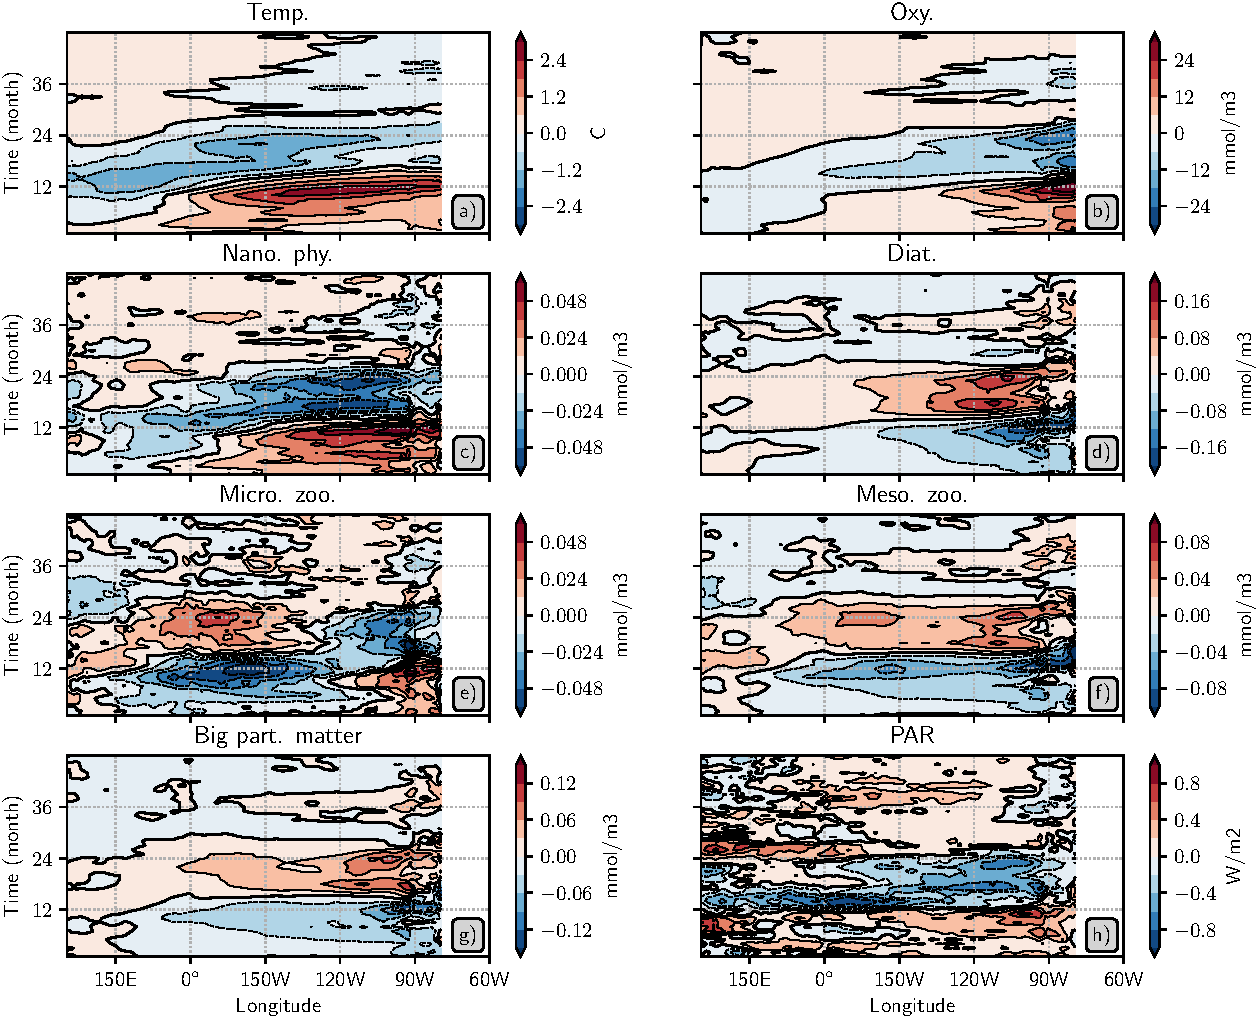
\includegraphics[scale=0.5]{figs/composite_hov_pisces.pdf}
    \caption{\hov\ diagrams of NEMO-Pisces variables averaged over the top 200m and between 2N and 2S. Month values of 10 to 12 indicate the onset of \nino\ conditions.}
    \label{fig:hov-pisces}
    \end{center}
\end{figure}

\clearpage
